\section{機器監視サービスの構成}
%(どのような要素で構成されているのか、また、それぞれの役割は何なのか)
%1.1全体構成(どのような要素で構成され、また、それぞれの役割について簡潔に述べる)
第3章にて述べた要件に基づき、システムを構築した。
システムは、エージェントプログラム、機器状態データベース、機器情報データベース、「かおりちゃん」というエージェントプログラム用インターフェースプログラム、Webアプリケーションサーバ、Webアプリケーションから成り立っている。
エージェントプログラムと「かおりちゃん」、WebアプリケーションサーバとWebアプリケーションは、インターネットを介して通信しあう。
\medskip

\begin{figure}[htbp]
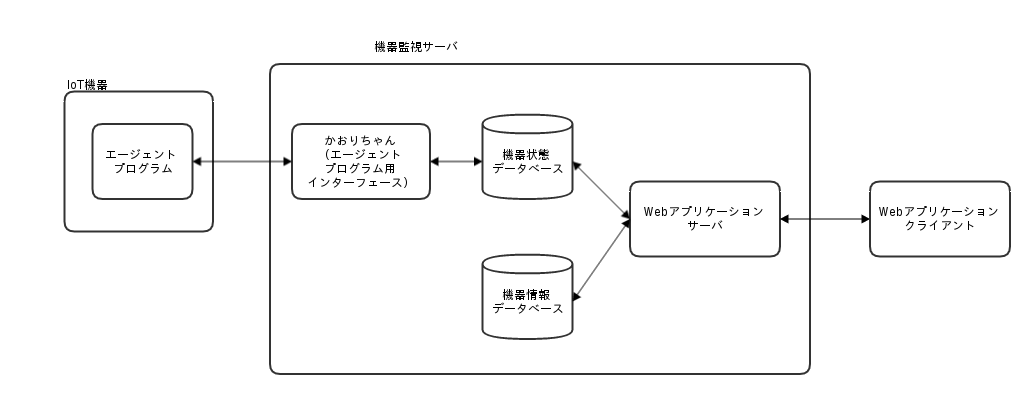
\includegraphics[width=16cm]{images/blockdiagram2.png}
\caption{システムのブロック図}
\label{fig:blockdiagram}
\end{figure}

エージェントプログラムは、IoT機器上で動作するプログラムである。
定期的に自身の状態を検知し、状態蓄積システムへ送信する役割を果たす。
定期的かつ自発的に状態を送信することで、ネットワーク環境によらない機器の監視を可能にした。
\medskip

「かおりちゃん」とは、エージェントプログラム用インターフェースである。
各IoT機器上で動くエージェントプログラムから送られてきた状態を、時刻と共に機器状態データベースへ書き込む役割を果たすプログラムで、機器監視サーバー上で動作する。
\medskip

機器状態データベースとは、機器の状態を時系列に沿って蓄積するデータベースである。
機器監視サーバー上で動作する。
\medskip

機器情報データベースとは、機器IDや、機器名、ユーザー名を記録するデータベースである。
機器監視サーバー上で動作する。
\medskip

Webアプリケーションとは、ユーザーからの入力を受けユーザーへ表示する他必要な情報を問い合わせる、ブラウザ上で動作するプログラムである。
\medskip

Webアプリケーションサーバーは、WebページやWebアプリケーション自体を配信する。
Webアプリケーションからの要求に答え、現在の機器の状態や、機器名等を返答する。
\medskip

これら各要素が連携することで、機器の監視を容易なものとした。

\subsection{エージェントプログラム}
%(エージェントプログラムとは何なのか)
エージェントプログラムとは、IoT機器上にインストールされるプログラムである。
エージェントプログラムの役割は、自身の状態を検知・記録し、送信失敗回数と共に「かおりちゃん」へ報告することである。
送信失敗回数とは、ネットワークの不具合等により、機器監視サーバーへ送信されなかった報告の数である。
自発的に状態を報告するため、IoT機器にプライベートアドレスが付与されていても、状態を検知することができる。
また、HTTPを用いるため、間のネットワークにてブロックされることがない。

\subsection{「かおりちゃん」}
かおりちゃんとは、エージェントプログラム用インターフェースで、サーバー上で動くプログラムである。
かおりちゃんの役割は、エージェントプログラムから送信された各機器の状態を、時刻と共に機器状態データベースへ書き込む事である。
また、エージェントプログラムから送られた送信失敗回数から、IoT機器がインターネットから切断された時刻を逆算し、機器状態データベースへ書き込む事も行う。


\subsection{機器状態データベース}
%(とは何なのか)
機器状態データベースとは、サーバ上で動作するデータベースである。
各IoT機器の状態を時刻とともに記録する。
機器状態監視システムの中心にあるデータベースである。

\subsection{機器情報データベース}
機器情報データベースとは、サーバー上で動作するデータベースである。
各IoT機器の機器ID、機器名、機器詳細情報、ユーザーのメールアドレスとパスワードを記録する。

\subsection{Webアプリケーションサーバ}
Webアプリケーションサーバとは、サーバ上で動作するプログラムである。
WebアプリケーションやWebページの配信、Webアプリケーションからの要求の処理などを行う。
必要に応じて、機器状態データベースと機器情報データベースへアクセスを行う。
次に、Webアプリケーションとのインターフェースを挙げ、それぞれについて説明する。
\subsubsection{ログインAPI}
Webアプリケーションから、メールアドレスとパスワードを受け取り、	機器情報データベースのユーザーテーブルと照合する。
照合した結果、ユーザー名とパスワードが合致したユーザーが存在すれば、HTTPクッキーにセッションキーをセットし、機器状態一覧ページへのリダイレクトを返す。
合致したユーザーが存在しなかった場合、エラーメッセージを返す。
\subsection{ログアウトAPI}
Webアプリケーションに、HTTPクッキーから該当のセッションキーを削除するよう要求する。
\subsubsection{機器情報・機器状態取得API}
ログインチェックを行った後、機器情報データベースと機器状態データベースより、全IoT機器の機器情報と機器状態を返す。
\subsubsection{機器ID生成API}
ログインチェックを行った後、機器情報データベースに存在しない、ランダムな機器IDを返す。
\subsubsection{機器ID重複チェックAPI}
ログインチェックを行った後。Webアプリケーションから機器IDを受け取る。
機器情報データベースに該当の機器IDが存在するかしないかを返す。
\subsubsection{機器作成API}
ログインチェックを行った後、Webアプリケーションから、機器ID、機器名、機器の詳細と、機器の作成なのか編集なのかの指示を受け取る。
機器の作成であった場合、
機器IDに重複が無いことを確認したうえで、機器情報データベースに該当のエントリを作成・機器状態データベースにメジャーメントを作成する。
作成されたか、されなかったかを返す。
機器の編集であった場合、
機器情報データベースから、受け取った機器IDを持つものを探しだし、編集する。
編集できたか否かを返す。
\subsubsection{機器削除API}
ログインチェックを行った後、Webアプリケーションから、機器IDを受け取る。
機器情報データベースから、受け取った機器IDを持つものを削除する。
その後、機器状態データベースから、メジャーメントを削除する。
削除されたか否かを返す。
\subsubsection{過去の機器状態取得API}
ログインチェックを行った後、機器状態データベースから、全てのIoT機器の過去の状態をまとめ、返す。

\subsection{Webアプリケーション}
Webアプリケーションとは、ユーザーのブラウザ上で動作するアプリケーションである。
ユーザーへグラフィカルインターフェースを提供する。
必要に応じて、Webアプリケーションサーバへ必要な情報を要求する。
Webアプリケーションは、3つのWebページから成り立っている。
以下に各ページとそれぞれの役割を述べる。
\begin{itemize}
	\item ログインページ\\
		正当なユーザーであることを確認するために、メールアドレスとパスワードの入力を求める。
		メールアドレスとパスワードは、Webアプリケーションサーバーへ送信される。
	\item 機器状態一覧ページ\\
		機器状態を一覧して表示する他、機器の作成や、機器情報の編集、機器の削除等を行う事ができる。
		現在の機器の状態を取得するため、定期的にWebアプリケーションサーバと通信する。
		また、機器の作成や機器情報の編集、削除の為、Webアプリケーションサーバと通信する。
	\item 過去の機器状態一覧ページ\\
		過去の機器状態を時刻と共に整理し、一覧表示するページである。
		現在の機器の状態を取得するため、定期的にWebアプリケーションサーバと通信をする。
\end{itemize}

\section{エージェントプログラムの実装}
エージェントプログラムの役割は、定期的にIoT機器の状態を検知し、IoT機器監視サーバーに送信することである。
約1分おきに、自身が稼働している事を示すメッセージと送信失敗回数を、「かおりちゃん」へ送信する。
どのようなLinux環境でも動作することを考え、Shellスクリプトにて実装した。

\section{「かおりちゃん」の実装}
「かおりちゃん」の役割は、エージェントプログラムから送信された各機器の状態を、時刻と共に機器状態データベースへ書き込むことと、
エージェントプログラムから送られた送信失敗回数から、インターネットより切断された時刻を逆算し、機器状態データベースへ書き込む事である。
Falconと呼ばれるAPIの作成に特化したフレームワークを使用し、Pythonにて実装した。

\section{機器情報データベース}
機器情報データベースの役割は、機器の名前、機器の詳細説明、機器ID、ログイン用ユーザーIDとパスワードを記録し保持する事である。
機器情報データベースには、SQLitei3を用いた。
機器情報データベースには、次のようなテーブルが用意されている。
\subsection{機器情報テーブル}
機器ID、ユーザーIDをキーとして、機器の名前、機器の詳細説明を記録し保持するテーブルである。
\subsection{ユーザーテーブル}
ユーザーIDをキーとして、ユーザー名とパスワードを記録し保持するテーブルである。

\section{機器状態データベース}
機器状態データベースの役割は、機器の状態を時刻と共に記録・保持することである。
機器状態データベースには、Influxdbを用いた。
機器IDをメトリクス名(テーブル名)とし、時刻をキーとして、機器の状態を記録している。

\section{Webサーバーアプリケーション}
Webサーバーアプリケーションの役割は、与えられたHTTPリクエストを元に、Webアプリケーション本体や、各種情報を返却することにある。
Flaskと呼ばれるWebアプリケーションフレームワークを用いた。Pythonを使用している。

\section{Webクライアントアプリケーション}
Webクライアントアプリケーションの役割は、ユーザーインターフェースを提供することである。
Bootstrap,JQueryというライブラリを用いて作成した。HTML,CSS,Javascriptで書かれている。
定期的にWebアプリケーションサーバから状態を取得し、HTML,CSSを用いて表示する。

\section{エージェントプログラムと「かおりちゃん」間の通信の実装}
%このような形式で、どんな情報を伝えているのか。
%特徴としてどのような事があるのか


\section{WebアプリケーションサーバとWebアプリケーション間の通信の実装}
%どのような形式で、どのような情報を伝えているのか。


\begin{comment}
URLの設計として次のようになっている。
\begin{description}
	\item[GET /login]\mbox{}\\
		ログインページを返す。
	\item[POST /login]\mbox{}\\
		メールアドレスとパスワードを受け取る。\\
		クッキーからセッションキーを探し、存在すれば既にログインしているとして、/dashboardへのリダイレクトメッセージを返す。
		データベースにメールアドレスとパスワードの組が存在するか確認し、存在した場合、セッションキーを返す。\\
		存在しなかった場合、ログインエラーページを返す。
	\item[GET /logout]\mbox{}\\
		セッションキーを受け取り、該当のセッションを削除する。\\
	\item[GET /dashboard]\mbox{}\\
		ログインチェックをし、機器状態一覧ページを返す。
	\item[GET /devicelog]\mbox{}\\
		ログインチェックをし、過去の機器状態一覧ページを返す。
	\item[GET /api/device/all]\mbox{}\\
		ログインチェックをし、現在の状態、最後にメッセージを受け取った日時、機器ID、機器名、機器詳細のデータを、JSON形式にまとめたものを返す。
	\item[GET /api/deviceID]\mbox{}\\
		ログインチェックをし、ランダムにデバイスIDを生成し、JSON形式にまとめたものを返す。
	\item[POST /api/deviceID]\mbox{}\\
		ログインチェックをし、受け取ったデバイスIDが既に存在するか確認し、その結果をJSON形式にまとめ、返す。
	\item[POST /api/device/\{DeviceID\}]\mbox{}\\
		ログインチェックをし、デバイスIDと受け取ったJSONデータから、デバイスの新規作成・編集をし、結果をJSON形式にまとめ、返す。
	\item[DELETE /api/device/\{DeviceID\}]\mbox{}\\
		ログインチェックをし、該当のデバイスIDを持つデバイスをデータベースから削除する。	
\end{description}

\subsection{「かおりちゃん」とエージェントプログラムの通信}
\subsection{WebアプリケーションサーバとWebアプリケーションの通信}
\end{comment}
